\section{Data Understanding}

\subsection{Dataset Description}

The main dataset is the MIT-BIH Arrhythmia Database from PhysioNet~\cite{moody2001mitbih}, the standard benchmark for beat classification, which allows comparison with published results.

\begin{table}[H]
  \centering
  \caption{Overview of the MIT-BIH Arrhythmia Database.}
  \label{tab:dataset}
  \rowcolors{2}{white}{rowtint}
  \begin{tabularx}{\linewidth}{l Y}
        \rowcolor{primaryblue}
    \hd{Property} & \hd{Value} \\
    Database           & MIT-BIH Arrhythmia Database, PhysioNet, version 1.0.0 \\
    Records            & 48 \\
    Subjects           & 47 (records 201 and 202 are from the same person) \\
    Channels           & 2 per record \\
    Sampling frequency & 360\,Hz \\
    Resolution         & 11 bits over a 10\,mV range \\
    Duration           & About 30 minutes per record, about 24 hours in total \\
    Annotations        & Beat-by-beat labels on the R-peak, made by two cardiologists with disagreements resolved \\
    Beat annotations   & About 110\,000 \\
    ECG leads          & First channel is modified limb lead II (MLII) in 46 records; second channel is usually V1, sometimes V2, V4 or V5. Records 102 and 104 have no MLII. \\
    \bottomrule
  \end{tabularx}

\end{table}

The recordings were made at Beth Israel Hospital in Boston between 1975 and 1979. Twenty-three records were selected at random from routine Holter tapes and twenty-five were selected because they contain rare but clinically important rhythms, which is why the database contains a usable number of abnormal beats despite its size.

For the noise experiment we use the MIT-BIH Noise Stress Test Database from the same source~\cite{moody1984noise}. It provides three half-hour recordings of pure noise, made with real electrodes on moving volunteers: baseline wander (\texttt{bw}), electrode motion artefact (\texttt{em}) and muscle artefact (\texttt{ma}). They are sampled at 360\,Hz, so they can be added directly to the arrhythmia recordings.

\subsection{Target Classes}

The database uses about fifteen beat symbols. They are grouped into the four required classes following the AAMI EC57 standard, which is also the grouping used in most inter-patient studies. Table~\ref{tab:classes} lists the mapping and the beat counts over the 44 records used.

\begin{table}[H]
  \centering
  \caption{Mapping from MIT-BIH beat symbols to the four target classes. Counts are produced by \texttt{prepare\_data.py} and stored in \texttt{results/split\_stats.csv}.}
  \label{tab:classes}
  \rowcolors{2}{white}{rowtint}
  \begin{tabularx}{\linewidth}{c l Y r}
        \rowcolor{primaryblue}
    \hd{Class} & \hd{MIT-BIH symbols} & \hd{Meaning} & \hd{Beats} \\
    N & \texttt{N}, \texttt{L}, \texttt{R}, \texttt{e}, \texttt{j} & Normal beat; left and right bundle branch block beats; atrial and nodal escape beats & 90\,125 \\
    S & \texttt{A}, \texttt{a}, \texttt{J}, \texttt{S}             & Atrial premature; aberrated atrial premature; nodal premature; supraventricular premature beats & 2\,781 \\
    V & \texttt{V}, \texttt{E}                                     & Premature ventricular contraction; ventricular escape beat & 7\,009 \\
    F & \texttt{F}                                                 & Fusion of ventricular and normal beat & 803 \\
    \bottomrule
  \end{tabularx}

\end{table}

\textbf{Excluded annotations.} Three kinds of labels are dropped. The preprocessing script counts every dropped beat, so the exclusions are reproducible.

\begin{itemize}[nosep]
  \item \textbf{Paced beats} (\texttt{/}) and \textbf{fusion of paced and normal beats} (\texttt{f}). These come from patients with pacemakers. The four paced records (102, 104, 107 and 217) are excluded entirely, as is standard practice, because the pacemaker spike is an artificial signal unrelated to the heart's own rhythm.
  \item \textbf{Unclassifiable beats} (\texttt{Q}). The annotators could not assign a class, so they cannot serve as training targets.
  \item \textbf{Non-beat annotations}, such as rhythm changes (\texttt{+}), noise markers (\texttt{\textasciitilde}) and signal-quality flags. These describe the recording, not a heartbeat, and are never counted as beats.
\end{itemize}

Excluding the paced records leaves 44 records, split evenly into DS1 and DS2 as described in Section~\ref{sec:record-selection}.

\subsection{Exploratory Data Analysis}

The full analysis is in \texttt{notebooks/EDA.ipynb}. The figures below summarise the main findings.

\textbf{The raw signal.} Figure~\ref{fig:raw-ecg} shows ten seconds of record 100, both channels. The MLII channel has a tall, sharp QRS complex on every beat, which makes it the preferred lead for beat analysis. The V1 channel shows the same beats with a smaller, partly inverted QRS.

\begin{figure}[H]
  \centering
  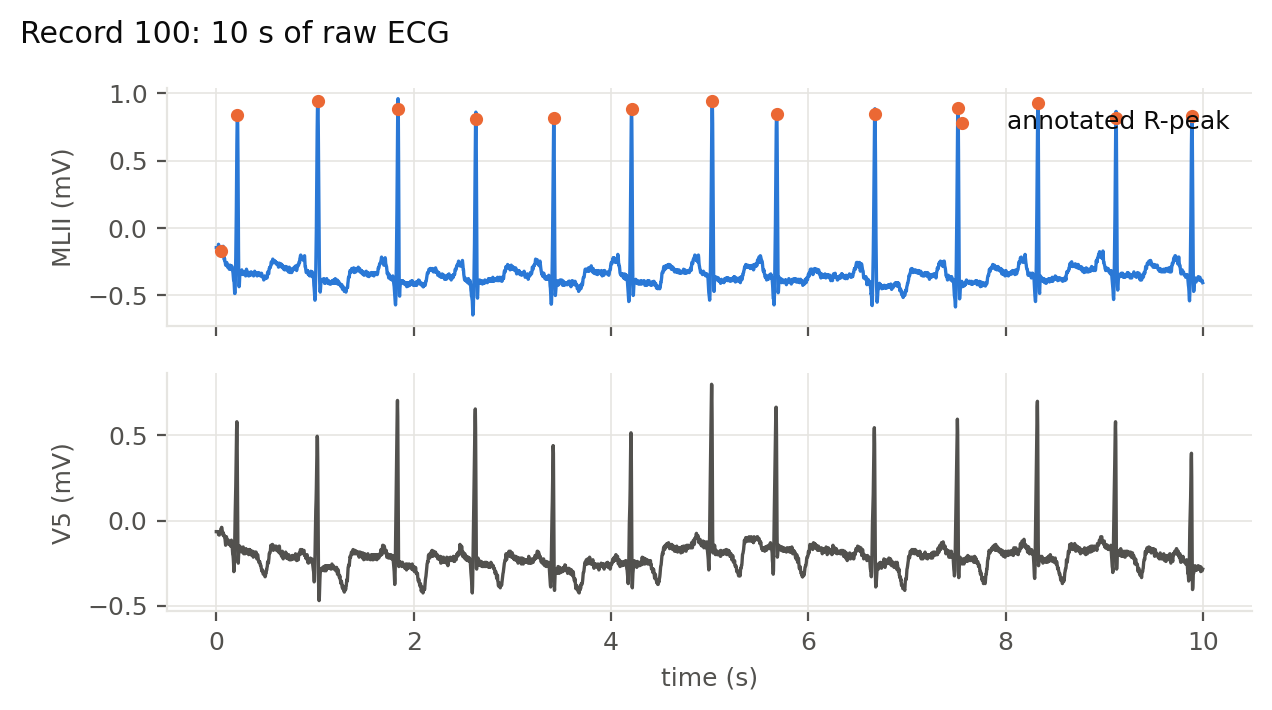
\includegraphics[width=\linewidth]{eda_raw_ecg.png}
  \caption{Ten seconds of raw ECG from record 100.}
  \label{fig:raw-ecg}
\end{figure}

\textbf{One beat per class.} Figure~\ref{fig:class-examples} shows a typical beat of each class, aligned on the R-peak. N and S beats are difficult to separate by shape; the main difference is timing, since the S beat arrives earlier than expected. The V beat has a wide QRS and no normal P wave. The F beat has an intermediate shape between N and V.

\begin{figure}[H]
  \centering
  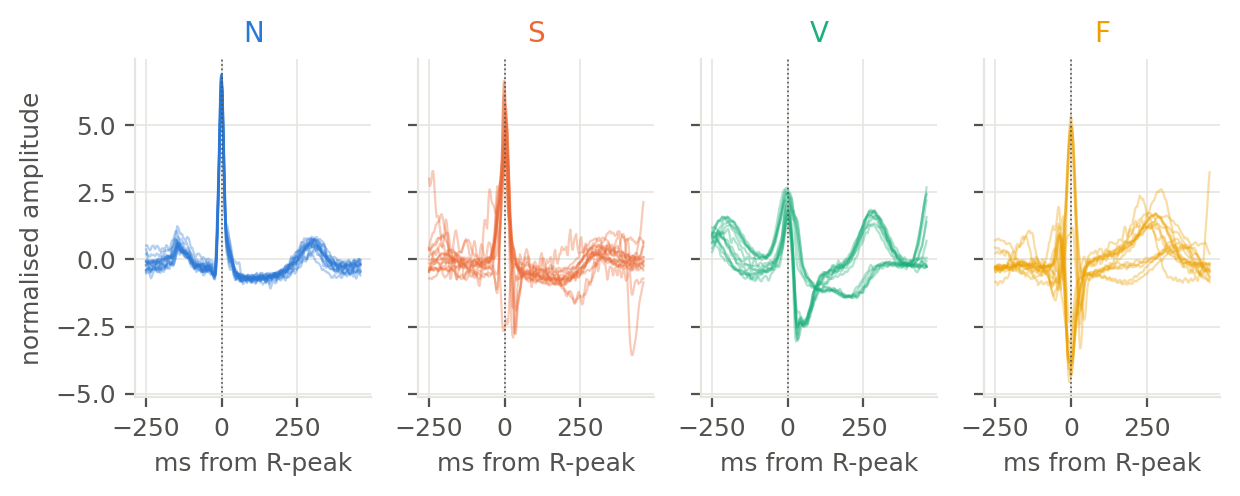
\includegraphics[width=\linewidth]{eda_class_examples.png}
  \caption{Example heartbeat of each class, 256-sample window centred on the R-peak.}
  \label{fig:class-examples}
\end{figure}

\textbf{Class distribution.} Figure~\ref{fig:class-dist} shows how uneven the classes are. Normal beats make up close to 90\,\% of the data, V beats are the largest minority, S beats are about 2--3\,\% and F beats well under 1\,\%. This imbalance motivates several decisions in Section~\ref{sec:data-preparation}.

\begin{figure}[H]
  \centering
  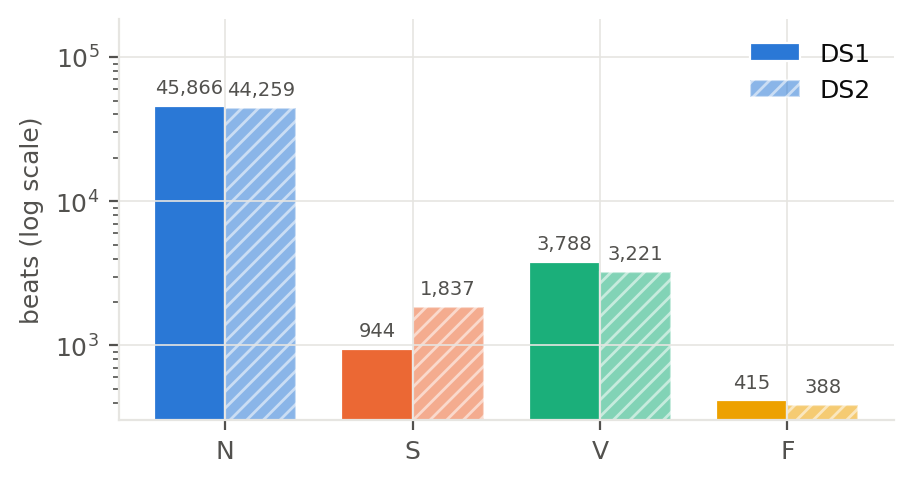
\includegraphics[width=\linewidth]{eda_class_distribution.png}
  \caption{Number of beats per class in DS1 and DS2 (logarithmic scale).}
  \label{fig:class-dist}
\end{figure}

\textbf{Beats per record.} Figure~\ref{fig:record-dist} shows the class composition of each record. The rare classes are not spread evenly: most S beats come from a few records such as 118, 207, 209 and 232, and most F beats from records 208 and 213. Performance on these classes therefore depends heavily on which records are in each split.

\begin{figure}[H]
  \centering
  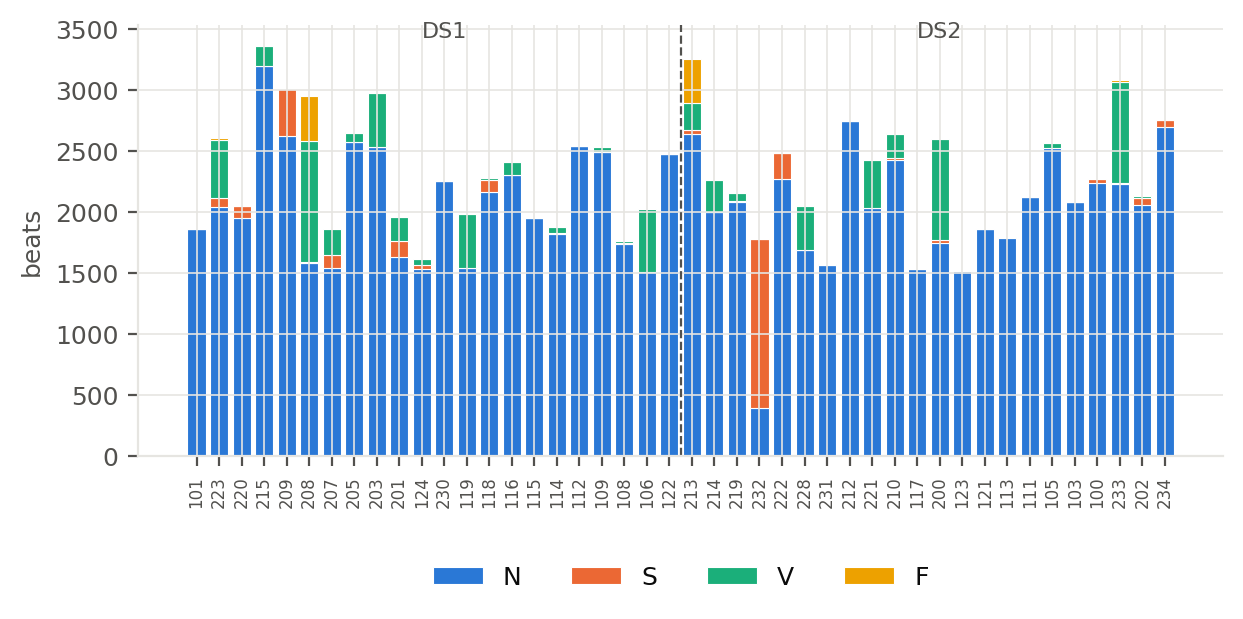
\includegraphics[width=\linewidth]{eda_record_distribution.png}
  \caption{Class composition of each record.}
  \label{fig:record-dist}
\end{figure}

\textbf{Signal amplitude.} Figure~\ref{fig:amplitude} shows the distribution of R-peak amplitude per record. Amplitudes vary by a factor of several between records because electrode placement and skin contact differ between subjects. Each beat is therefore normalised individually rather than with one global scale.

\begin{figure}[H]
  \centering
  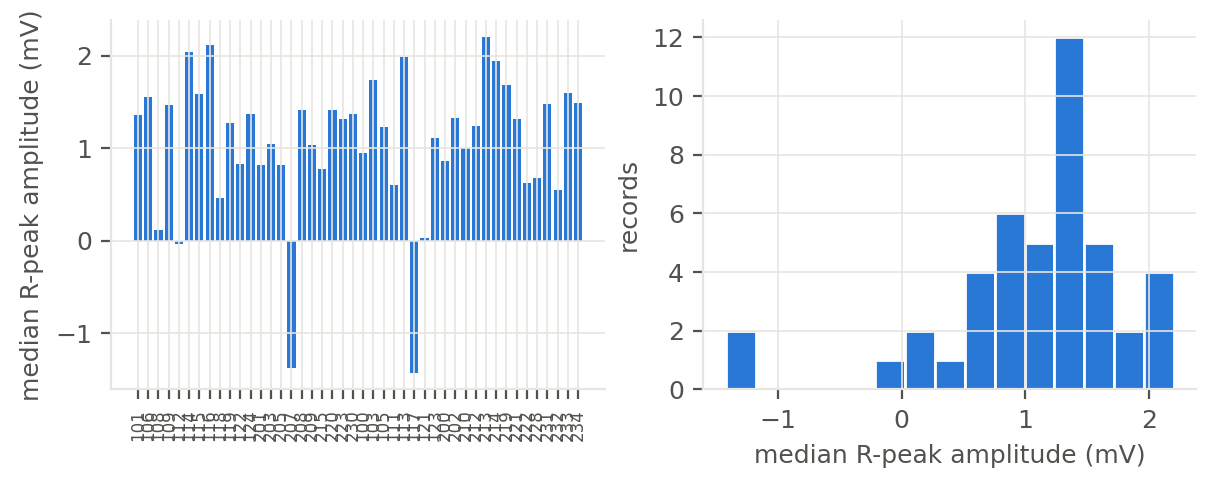
\includegraphics[width=\linewidth]{eda_amplitude.png}
  \caption{Distribution of R-peak amplitude across records.}
  \label{fig:amplitude}
\end{figure}

\textbf{Noisy ECG.} Figure~\ref{fig:noisy} shows segments from records 203 and 207, which are known to be noisy, together with the three noise types from the Noise Stress Test Database. Baseline wander is a slow drift, muscle artefact is high-frequency noise, and electrode motion produces abrupt transients that can resemble beats.

\begin{figure}[H]
  \centering
  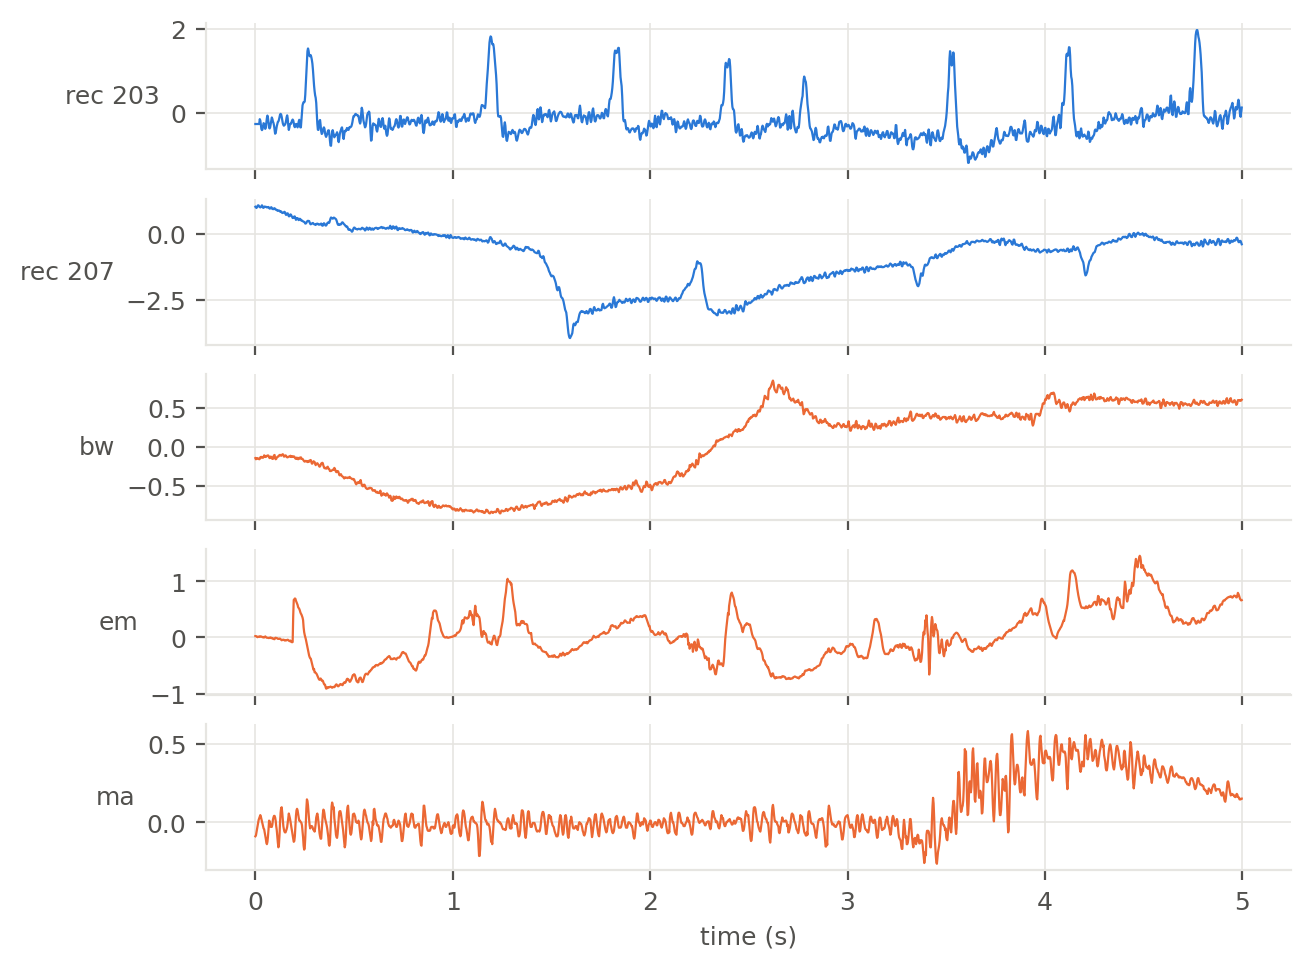
\includegraphics[width=\linewidth]{eda_noisy.png}
  \caption{Examples of noisy ECG and of the three noise types used in the robustness test.}
  \label{fig:noisy}
\end{figure}

\subsection{Data Quality}

\textbf{Missing data.} The recordings have no missing samples. Every record is complete at 360\,Hz.

\textbf{Extreme amplitudes.} A few records contain short bursts where the signal saturates at the limits of the 10\,mV range, usually during electrode movement. These segments are rare. Per-beat normalisation and clipping limit their effect on the input.

\textbf{Corrupted segments.} The annotators marked noisy stretches with the \texttt{\textasciitilde} symbol. Records 203, 207 and 208 contain the most of these. The beats inside these segments are kept, since a wearable will encounter the same kind of signal, but they are a likely source of label noise.

\textbf{Class imbalance.} Described above; it is the main data-quality issue.

\textbf{Differences between recordings.} Heart rate, beat shape, amplitude and noise level all vary from record to record. Some records show only normal rhythm, others show bundle branch block on every beat, and a few contain long runs of ventricular beats. Because of this variation, results on a small number of records can be misleading.

\textbf{Differences between channels.} MLII is the first channel in 46 of the 48 records, but in record 114 the two channels are stored in the opposite order. Selecting the lead by name rather than by column index avoids reading the wrong signal. Records 102 and 104 have no MLII; both are paced records and are already excluded.

\textbf{Possible noisy regions.} Baseline wander is present to some degree in almost every record. It is removed in preprocessing rather than detected and skipped.

\subsection{Leakage Analysis}

Data leakage occurs when information from the test set reaches the model during training, so the test score no longer measures generalisation.

A record is thirty minutes of ECG from one person. Its roughly 2\,000 beats share the same heart, electrodes and skin contact, so they are highly similar. If all beats were pooled, shuffled and split 80/20, nearly every test beat would have a near-duplicate in the training set. A model could then memorise each patient's waveform and exceed 99\,\% test accuracy without learning what distinguishes the classes. Studies using such splits report accuracies of this kind, which fall to 80--90\,\% when the same models are tested on unseen subjects. A wearable device only sees unseen subjects, so the shuffled score does not measure the quantity of interest.

Three measures prevent this. First, the data is split by record using the standard inter-patient partition: 22 records form the development set DS1 and 22 different records form the test set DS2, with no record in both. The partition has one known weakness: records 201 and 202 come from the same subject, and the standard split places 201 in DS1 and 202 in DS2. The partition is kept as published so that results remain comparable with the literature, and this is noted as a limitation. Second, the training/validation split inside DS1 is also by record, so model selection uses subjects the model was not trained on. Third, the split is enforced in code: the split-building function rejects a validation record that is not in DS1 and checks that no record is listed twice, and the evaluation script refuses to run on DS2 without an explicit \texttt{--final} flag. DS2 is used once per final model, after all design decisions are fixed.

The same rule applies to the noise experiment. Noise is added to DS2 only at evaluation time and the noisy signals are never used for training. Noise used as training augmentation is added to DS1 records only.
